\documentclass[10pt]{beamer}

\usepackage{appendixnumberbeamer}
\usepackage{booktabs}
\usepackage[scale=2]{ccicons}
\usepackage{pgfplots}
\usepackage{xspace}
\usepackage{bookmark}
\usepackage{amssymb}
\usepackage{mathtools}
\usepackage[normalem]{ulem}
\usepackage[T1]{fontenc}
\usepackage[sfdefault,book]{FiraSans}
\usepackage{FiraMono}
\usepackage{fontawesome}
\usepackage{hyperref}
\usepackage{listings}

\renewcommand{\thefootnote}{\fnsymbol{footnote}}
\renewcommand{\MintedPygmentize}{/home/thiago/.local/bin/pygmentize}

\definecolor{light-gray}{gray}{0.95}
\renewcommand\lstlistingname{Código}
\DeclareCaptionFormat{listing} {
  \parbox{\textwidth}{\hspace{-0.2cm}#1#2#3}
}
\DeclareCaptionFont{black}{\color{black}}
\captionsetup[lstlisting]{
  format=listing,
  labelfont=black,
  textfont=black,
  singlelinecheck=true,
  margin=0pt,
  font={tt,footnotesize,bf}
}

\lstset{
  basicstyle=\footnotesize\ttfamily,
  escapeinside={\%*}{*)},
  mathescape=true,
  showspaces=false,
  showtabs=false,
  showstringspaces=false,%
  rulesepcolor=\color{black},
  frame=shadowbox,
  upquote=true,
  literate=
  {á}{{\'a}}1 {é}{{\'e}}1 {í}{{\'i}}1 {ó}{{\'o}}1 {ú}{{\'u}}1
  {Á}{{\'A}}1 {É}{{\'E}}1 {Í}{{\'I}}1 {Ó}{{\'O}}1 {Ú}{{\'U}}1
  {à}{{\`a}}1 {è}{{\`e}}1 {ì}{{\`i}}1 {ò}{{\`o}}1 {ù}{{\`u}}1
  {À}{{\`A}}1 {È}{{\'E}}1 {Ì}{{\`I}}1 {Ò}{{\`O}}1 {Ù}{{\`U}}1
  {ä}{{\"a}}1 {ë}{{\"e}}1 {ï}{{\"i}}1 {ö}{{\"o}}1 {ü}{{\"u}}1
  {Ä}{{\"A}}1 {Ë}{{\"E}}1 {Ï}{{\"I}}1 {Ö}{{\"O}}1 {Ü}{{\"U}}1
  {â}{{\^a}}1 {ê}{{\^e}}1 {î}{{\^i}}1 {ô}{{\^o}}1 {û}{{\^u}}1
  {Â}{{\^A}}1 {Ê}{{\^E}}1 {Î}{{\^I}}1 {Ô}{{\^O}}1 {Û}{{\^U}}1
  {Ã}{{\~A}}1 {ã}{{\~a}}1 {Õ}{{\~O}}1 {õ}{{\~o}}1
  {œ}{{\oe}}1 {Œ}{{\OE}}1 {æ}{{\ae}}1 {Æ}{{\AE}}1 {ß}{{\ss}}1
  {ű}{{\H{u}}}1 {Ű}{{\H{U}}}1 {ő}{{\H{o}}}1 {Ő}{{\H{O}}}1
  {ç}{{\c c}}1 {Ç}{{\c C}}1 {ø}{{\o}}1 {å}{{\r a}}1 {Å}{{\r A}}1
  {€}{{\euro}}1 {£}{{\pounds}}1 {«}{{\guillemotleft}}1
  {»}{{\guillemotright}}1 {ñ}{{\~n}}1 {Ñ}{{\~N}}1 {¿}{{?`}}1
}

\setminted{
  fontsize=\footnotesize,
  style=bw,
  frame=single,
  labelposition=topline,
}

\pretitle{\begin{center}\normalsize\bfseries\MakeUppercase{Programação 2 -- }\MakeUppercase}
\author{\normalsize Prof. Thiago Cavalcante}
\date{\vspace{-4ex}}

\geometry{
  top=0.0cm,
  left=1.0cm,
  right=1.0cm,
  bottom=1.0cm
}

\setlength\columnsep{30pt}

\usetikzlibrary{arrows}

\makeatletter
\AddEnumerateCounter{\PaddingUp}{\two@digits}{A00}
\AddEnumerateCounter{\PaddingDown}{\two@digits}{A00}
\newcommand\PaddingUp[1]{\expandafter\two@digits\csname c@#1\endcsname}
\newcommand\PaddingDown[1]{\PaddingUp{#1}\addtocounter{#1}{-2}}
\makeatother

\makeatletter
\def\enumalphalphcnt#1{\expandafter\@enumalphalphcnt\csname c@#1\endcsname}
\def\@enumalphalphcnt#1{\AlphAlph{#1}}
\makeatother
\AddEnumerateCounter{\enumalphalphcnt}{\@enumalphalphcnt}{aa}

\pagenumbering{gobble}

\title{Programação 2}
\author{Thiago Cavalcante  -- thiago.cavalcante@penedo.ufal.br}
\institute{Universidade Federal de Alagoas -- UFAL \\ Campus Arapiraca \\ Unidade de Ensino de Penedo}
\titlegraphic{\hfill
\includegraphics[height=1.5cm]{images/brasao-ufal.eps}}


\makeatletter
\newcommand\thefontsize[1]{{#1 The current font size is: \f@size pt\par}}
\makeatother

% \normalsize = 10.00pt
% \large      = 12.00pt
% \Large      = 14.40pt
% \LARGE      = 17.28pt
% \huge       = 20.74pt
% \Huge       = 24.88pt

\subtitle{Aula 3}
\date{06 de novembro de 2019}

\begin{document}

\maketitle

\begin{frame}{Funções}
  \huge
  \textbf{Bloco de código} que pode ser \textbf{nomeado} e \textbf{chamado} dentro de um programa
  \vfill
  \LARGE
  Exemplos: \texttt{scanf()} e \texttt{printf()}
\end{frame}

\begin{frame}{Funções}
  \huge
  \textbf{Por que usar funções?}
  \vfill
  \begin{itemize}
    \item Estruturação do programa
    \item Reutilização de código
  \end{itemize}
\end{frame}

\begin{frame}[fragile]{Funções}
  \huge
  \textbf{Declarando uma função}
  \vfill
  \large
  \begin{verbatim}
tipo_retornado nome_função(parâmetros) {
    declarações e comandos
}
  \end{verbatim}

  Nome da função segue regras de nome de variáveis
\end{frame}

\begin{frame}[fragile]{Funções}
  \huge
  \textbf{Local da declaração}
  \vfill
  \large
  \begin{enumerate}
    \item Declaração antes da \textbf{\texttt{main()}}
    \item Protótipo antes da \textbf{\texttt{main()}} e declaração depois
  \end{enumerate}
  \vfill
  \large
  O protótipo contém apenas o \textbf{cabeçalho} da função
\end{frame}

\begin{frame}{Funções}
  \huge
  \textbf{Funcionamento de uma função}
  \vfill
  \Large
  \begin{itemize}
    \item Fluxo do programa é interrompido
    \item Valores são copiados para parâmetros
    \item Comandos da função são executados
    \item Valor do \texttt{\textbf{return}} é copiado para variável
    \item Fluxo do programa continua
  \end{itemize}
\end{frame}

\begin{frame}[fragile]{Funções}
  \huge
  \textbf{Lista de parâmetros}
  \vfill
  \large
  \begin{verbatim}
(tipo1 nome1, tipo2 nome2, ..., tipoN nomeN)
  \end{verbatim}
  \vfill
  \setlength{\leftmargini}{0pt}
  \begin{itemize}
      \item [] o tipo deve vir antes de \textbf{cada} parâmetro, mesmo se os tipos forem iguais (ex.: \texttt{int x, int y})
      \item [] o parâmetro só pode ser acessado \textbf{dentro} da função
  \end{itemize}
\end{frame}

\begin{frame}[fragile]{Funções}
  \huge
  \textbf{A lista \alert{não é obrigatória}}
  \vfill
  \Large
  \begin{columns}
    \begin{column}{0.35\textwidth}
      \begin{lstlisting}
tipo nome%*\textbf{()}*) {
  ...
}
      \end{lstlisting}
    \end{column}
    \begin{column}{0.60\textwidth}
      \begin{lstlisting}
|
|  tipo nome%*\textbf{(void)}*) {
|    ...
|  }
|
      \end{lstlisting}
    \end{column}
  \end{columns}
  \vfill
  \large
  Existe uma diferença entre as declarações
\end{frame}

\begin{frame}{Funções}
  \huge
  \textbf{Corpo da função}
  \vfill
  \LARGE
  \begin{itemize}
    \item Sequência de declarações
    \item Sequência de comandos
  \end{itemize}
  \vfill
  \large
  \setlength{\leftmargini}{0pt}
  \begin{itemize}
      \item [] A \textbf{\texttt{main()}} é uma função presente cada programa
      \item [] Tudo o que é feito na \textbf{\texttt{main()}} pode ser feito em outras funções
  \end{itemize}
\end{frame}

\begin{frame}{Funções}
  \huge
  Em geral, \textbf{evita-se fazer leitura e escrita} de dados dentro de uma função
  \vfill
  Uma possível exceção: \textbf{menu de usuário}
\end{frame}

\begin{frame}[fragile]{Funções}
  \huge
  \textbf{Retorno da função}
  \vfill
  \Large
  \begin{verbatim}
    return expressão;
      \end{verbatim}
  \vfill
  \large
  Uma função pode retornar \textbf{qualquer um} dos tipos válidos em C (incluindo tipos definidos pelo usuário)
\end{frame}

\begin{frame}{Funções}
  \huge
  \textbf{Retorno da função}
  \vfill
  \Large
  Uma função pode \textbf{não retornar} nada também, basta definir o \texttt{tipo\_retornado} como \textbf{\texttt{void}}
  \vfill
  \large
  Exemplo: uma função para imprimir algo na tela
\end{frame}

\begin{frame}{Funções}
  \huge
  Uma função pode retornar:
  \vfill
  \Large
  \begin{itemize}
    \item Variável
    \item Constante
    \item Expressão artimética
    \item Expressão lógica
    \item Outra função
  \end{itemize}
  \vfill
  \large
  O retorno precisa ser compatível com o tipo definido
\end{frame}

\begin{frame}[fragile]{Funções}
  \huge
  Uma função pode ter \textbf{vários} comandos \texttt{return}
  \vfill
  \normalsize
  \begin{columns}
    \begin{column}{0.40\textwidth}
      \begin{lstlisting}

int max(int x, int y) {
  if(x > y)
    %*\textbf{return}*) x;
  else
    %*\textbf{return}*) y;
}

      \end{lstlisting}
    \end{column}
    \begin{column}{0.50\textwidth}
      \begin{lstlisting}
|  int max(int x, int y) {
|    int z;
|    if(x > y)
|      z = x;
|    else
|      z = y;
|    %*\textbf{return}*) z;
|  }
      \end{lstlisting}
    \end{column}
  \end{columns}
\end{frame}

\begin{frame}{Funções}
  \large
  \begin{itemize}
    \item A função \textbf{encerra} quando chega em um \textbf{\texttt{return}}
    \item Uma função do tipo \textbf{\texttt{void}} pode ser finalizada com \textbf{\texttt{return;}}
    \item Uma função \textbf{não pode} retornar um \textbf{array} (a não ser que esteja dentro de uma \texttt{struct})
  \end{itemize}
\end{frame}

\begin{frame}{Funções}
  \huge
  \textbf{Passagem de parâmetros}
  \vfill
  \begin{itemize}
    \item Por \textbf{valor}
    \item Por \textbf{referência}
  \end{itemize}
\end{frame}

\begin{frame}{Funções}
  \huge
  Passagem por \textbf{valor}
  \vfill
  \Large
  \begin{itemize}
    \item O argumento é \textbf{copiado} para o parâmetro
    \item O parâmetro é uma \textbf{variável local} da função
    \item Mudanças no parâmetro \textbf{não refletem} no argumento
    \item O parâmetro é \textbf{destruído} e o argumento mantém seu valor \textbf{original}
  \end{itemize}

\end{frame}

\begin{frame}[fragile]{Funções}
  \huge
  Passagem por \textbf{referência}
  \vfill
  \large
  \begin{itemize}
    \item Usada quando se quer \textbf{alterar} o valor do argumento
    \item Não é passado o valor da variável, mas sim o seu \textbf{endereço na memória}
    \item Na \textbf{declaração} e \textbf{corpo} da função, usa-se o operador \textbf{\texttt{*}} antes da variável
    \item Na \textbf{chamada} da função, usa-se o operador \textbf{\&} antes da variável
  \end{itemize}
  \vfill
  \large
  Exemplo: \texttt{scanf("\%d", }\&\texttt{x);}
\end{frame}

\begin{frame}{Funções}
  \huge
  \textbf{Passagem de arrays como parâmetros}
  \vfill
  \Large
  \begin{itemize}
    \item Arrays são \textbf{sempre} passados \textbf{por referência}
    \item É necessário sempre um segundo parâmetro contendo o \textbf{tamanho} do array
  \end{itemize}

\end{frame}

\begin{frame}{Funções}
  \huge
  \textbf{Declarando os parâmetros}
  \vfill
  \LARGE
  \begin{itemize}
    \item \texttt{int *array, int tamanho}
    \item \texttt{int array[], int tamanho}
    \item \texttt{int array[5], int tamanho}
  \end{itemize}
  \vfill
  \large
  Os primeiros elementos são todos equivalentes, pois o tamanho não é checado
\end{frame}

\begin{frame}[fragile]{Funções}
  \LARGE
  Não é necessário usar o operador \& na \textbf{chamada} da função para um array, pois o seu \textbf{nome representa o endereço do seu primeiro elemento} na memória
  \vfill
  \begin{lstlisting}
array = %*\textnormal{\&}*)array[0]
  \end{lstlisting}
\end{frame}

\begin{frame}[fragile]{Funções}
  \LARGE
  Não é necessário usar o operador \texttt{*} no \textbf{corpo} da função para um array. O \textbf{acesso aos seus elementos pode ser feito normalmente} com colchetes.
  \vfill
  \begin{lstlisting}
x = array[elemento];
  \end{lstlisting}
\end{frame}

\begin{frame}[fragile]{Funções}
  \huge
  \textbf{Arrays multidimensionais}
  \vfill
  \Large
  É necessário indicar o tamanho das dimensões extras na declaração da função.
  \vfill
  \begin{verbatim}
int array[][5], int tamanho
  \end{verbatim}

\end{frame}

\begin{frame}{Funções}
  \huge
  \textbf{Passagem de structs como parâmetros}
  \vfill
  \Large
  \begin{itemize}
    \item Passagem por \textbf{valor}

    \begin{itemize}
      \Large
      \item estrutura
      \item campo da estrutura
    \end{itemize}
    \item Passagem por \textbf{referência}

    \begin{itemize}
      \Large
      \item estrutura
      \item campo da estrutura
    \end{itemize}
  \end{itemize}
\end{frame}

\begin{frame}[fragile]{Funções}
  \huge
  \textbf{Operador seta}
  \vfill
  \large
  Quando a estrutura é passada por referência, o acesso a ela dentro da função pode ser feito com os operadores \textbf{\texttt{*}} e \textbf{.} em conjunto ou com o operador \textbf{\texttt{->}}
  \vfill
  \large
  \begin{verbatim}
(*struct).campo
struct->campo
  \end{verbatim}
\end{frame}

\begin{frame}{Funções}
  \huge
  \textbf{Recursão (definição circular)}
  \vfill
  \centering
  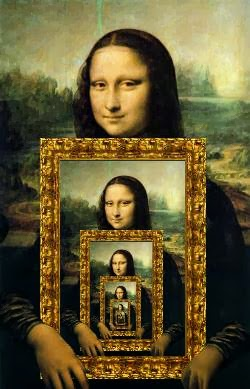
\includegraphics[height=.7\textheight]{images/recursao.jpg}
\end{frame}

\begin{frame}{Funções}
  \huge
  Uma \textit{funçao recursiva} \textbf{chama a si própria} dentro da sua definição.
\end{frame}

\begin{frame}{Funções}
  \Huge
  Exemplo clássico: \textbf{fatorial}
\end{frame}

\begin{frame}{Funções}
  \huge
  \textbf{Como funciona a recursividade}
  \vfill
  \LARGE
  \begin{itemize}
    \item Dividir e conquistar
    \item Caminho de ida $\rightarrow$ caso-base $\rightarrow$ caminho de volta
  \end{itemize}

\end{frame}

\begin{frame}{Funções}
  \huge
  \textbf{Cuidados a serem tomados}
  \vfill
  \LARGE
  \begin{itemize}
    \item Critério de parada
    \item Parâmetro da chamada recursiva
  \end{itemize}
\end{frame}

\begin{frame}{Funções}
  \LARGE
  Algoritmos recursivos são \textbf{considerados mais enxutos/elegantes}, porém \textbf{tendem a ser mais ineficientes} (tempo/memória) e apresentam maior dificuldade na detecção de erros
  \vfill
  Ex.: \textbf{Fibonacci}
\end{frame}

\end{document}
